In the course, we discussed the limitations of the binary cross entropy
loss (BCE Loss). It can lead to: 
\begin{itemize}
\item \href{https://developers.google.com/machine-learning/gan/problems}{mode collapse}: when the generator is stuck in a single mode of the distribution it is trying to replicate. For example, a generator training on the MNIST dataset would be stuck in generating images of certain digits only, as shown below.

    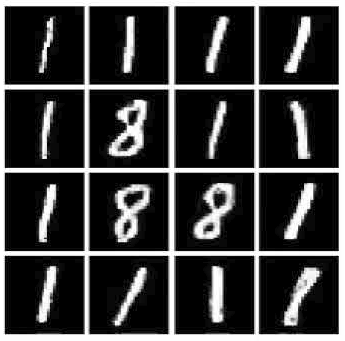
\includegraphics[width=0.5\linewidth]{img//genAdvNet//modernGAN/collapse.png}

\item vanishing gradient: it's a common problem with many neural networks architectures but is very common when training GANs. Because the discriminator's task is much easier than the generator's, the discriminator tends to converge faster and reach a high accuracy. The discriminator loss gets close to zero and the gradients become very small, leading to that vanishing gradient problem.
\end{itemize}

In this notebook, you will: 
\begin{itemize}
    \item implement the Wasserstein Loss
    \item implement two types of gradient penalties
\end{itemize}

\subsection{Wasserstein Loss}

The \href{https://arxiv.org/pdf/1701.07875.pdf}{Wasserstein GAN paper}
introduced a new type of loss function: the
\href{https://en.wikipedia.org/wiki/Wasserstein_metric}{Wasserstein
Distance}. We are now reshaping the problem GANs are solving: instead of
having a loss function that classifies a distribution as being real or
not, we have a loss function that tries to minimize the distance between
the real and the fake distribution. The difference is subtle but plays a
big role in the stability of GANs

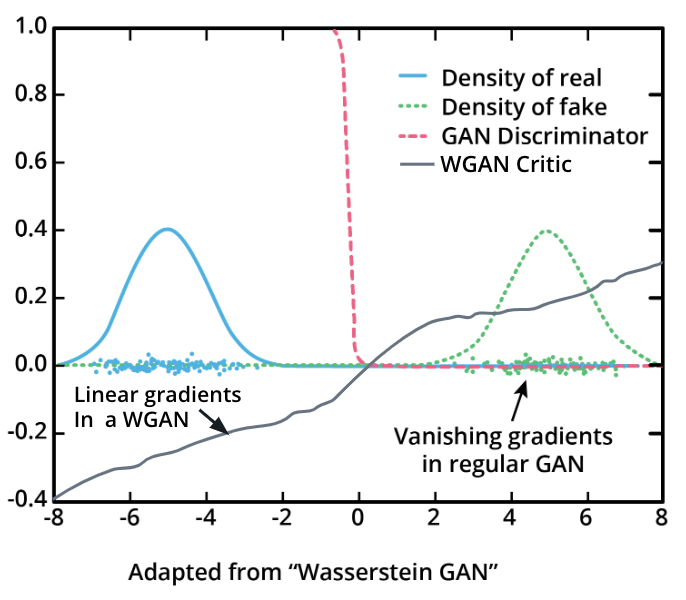
\includegraphics[width=0.75\linewidth]{img//genAdvNet//modernGAN/gradient_replace.png}

The discriminator is now called a \textbf{critic} because it's job is
not really to distinguish between real and fake anymore but to maximize
the distance between the two distributions. However, we will be using
both terms interchangeably for the sake of clarity. \newline

The Wasserstein loss can be calculated using the formula below:

\[\min_{g} \max_{c} E(c(x)) - E(c(g(z)))\]

You are now familiar with the minimax function. The main difference with
the BCE Loss is the disapperance of the logs!

\subsubsection{First exercise: implement the Wasserstein Loss}

The Wasserstein Loss (W-Loss) is taking the vector of logits outputed by
the discriminator as input. In comparison, the BCE Loss was taking the
probabilities (logits after a softmax layer) as inputs. The
discriminator W-Loss is trying to maximize the mean value of the logits
of real images and minize the mean value of the logits of fake images.
The generator W-Loss is trying to maximize the mean value of the logits
of fake images.

\begin{lstlisting}[language=Python]
import torch

import tests
\end{lstlisting}

\begin{lstlisting}[language=Python]
def disc_w_loss(real_logits: torch.Tensor, fake_logits: torch.Tensor):
    """
    Wasserstein Discriminator Loss
    
    args:
    - real_logits: vector of logits outputed by the discriminator with a real input image
    - fake_logits: vector of logits outputed by the discriminator with a fake input image 
    """
    real_loss = -real_logits.mean()
    fake_loss = fake_logits.mean()
    return real_loss + fake_loss
\end{lstlisting}

\begin{lstlisting}[language=Python]
def disc_g_loss(fake_logits: torch.Tensor):
    """
    Wasserstein Generator Loss
    
    args:
    - fake_logits: vector of logits outputed by the discriminator with a fake input image 
    """
    fake_loss = -fake_logits.mean()
    return fake_loss
\end{lstlisting}

\begin{lstlisting}[language=Python]
tests.check_disc_w_loss(disc_w_loss)
\end{lstlisting}

\begin{lstlisting}[language=Python]
tests.check_gen_w_loss(disc_g_loss)
\end{lstlisting}

\subsection{Gradient penalty}

To train a GAN with the Wasserstein Loss, the discriminator (or critic)
must be
\href{https://en.wikipedia.org/wiki/Lipschitz_continuity}{1-Lipschitz
continuous}. \newline

The 1-Lipschitz continuity constraint implies that the norm of the
gradient of the function must be below 1. In other words, for a function
\(f(x)\):

\[|| \frac{df}{dx} || < 1\]

Because the W-Loss is not bounded between 0 and 1 like the BCE loss, the
above constraint makes sure that the loss does not grow too much. \newline

In the original paper, the authors enforced this condition by using
weight clipping. However, per their own words:

\begin{lstlisting}
Weight clipping is a clearly terrible way to enforce a Lipschitz constraint. If the
clipping parameter is large, then it can take a long time for any weights to reach
their limit, thereby making it harder to train the critic till optimality. If the clipping
is small, this can easily lead to vanishing gradients when the number of layers is
big, or batch normalization is not used (such as in RNNs). We experimented with
simple variants (such as projecting the weights to a sphere) with little difference, and
we stuck with weight clipping due to its simplicity and already good performance.
However, we do leave the topic of enforcing Lipschitz constraints in a neural network
setting for further investigation, and we actively encourage interested researchers
to improve on this method.
\end{lstlisting}

\subsection{WGAN-GP}

Introducing Wasserstein Gan with Gradient Penalty, or
\href{https://arxiv.org/pdf/1704.00028.pdf}{WGAN-GP}. In this paper, the
author introduce a more robust way to enforce the 1-Lipschitz constaint
of the critic: a \textbf{gradient penalty term} in the loss function.
The new loss function is described below:

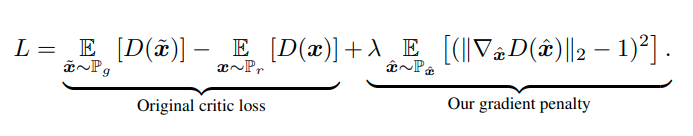
\includegraphics[width=1\linewidth]{img//genAdvNet//modernGAN/wgan_gp.png}

The gradient penalty is calculated as follow: 
\begin{itemize}
    \item sample a random point \(\hat{x}\) between the generated distribution and the real distribution.
    \item run this sample through the discriminator and calculate the gradient \(\nabla_{\hat{x}} D(\hat{x})\)
    \item calculate the L2 norm of the gradient \(|| \nabla_{\hat{x}} D(\hat{x}) ||_{2}\)
    \item remove 1, square the result and calculate the mean \((|| \nabla_{\hat{x}} D(\hat{x}) ||_{2} - 1) ^{2}\)
\end{itemize}

\subsubsection{Second exercise: implement the gradient penalty}
In the second exercise of this notebook, you will implement the above
gradient penalty. To help you, I have created a dummy critic module. \newline

\textbf{Tips}: 
\begin{itemize}
    \item to calculate the gradients, you first have to set the attribute of a tensor \lstinline{requires_grad} to True.
    \item you can use the following code to calculate the gradients:
\end{itemize}

\begin{lstlisting}
torch.autograd.grad(critic(x), x, grad_outputs=torch.ones_like(critic(x)), create_graph=True)[0]
\end{lstlisting}

\begin{lstlisting}[language=Python]
import torch.nn as nn
\end{lstlisting}

\begin{lstlisting}[language=Python]
class Critic(nn.Module):
    """ 
    Dummy critic class 
    """
    def __init__(self):
        super(Critic, self).__init__()
        
    def forward(self, x: torch.Tensor) -> torch.Tensor:
        return torch.pow(x, 2)
\end{lstlisting}

\begin{lstlisting}[language=Python]
def gradient_penalty(real_sample: torch.Tensor, 
                     fake_sample: torch.Tensor,
                     critic: nn.Module) -> torch.Tensor:
    """
    Gradient penalty of the WGAN-GP model
    args:
    - real_sample: sample from the real dataset
    - fake_sample: generated sample
    
    returns:
    - gradient penalty
    """
    # sample a random point between both distributions
    alpha = torch.rand(real_sample.shape)
    x_hat = alpha * real_sample + (1 - alpha) * fake_sample
    
    # calculate the gradient
    x_hat.requires_grad = True
    pred = critic(x_hat)
    grad = torch.autograd.grad(pred, 
                               x_hat, 
                               grad_outputs=torch.ones_like(pred), 
                               create_graph=True)[0]
    
    # calculate the norm and the final penalty
    norm = torch.norm(grad.view(-1), 2)
    gp = ((norm - 1)**2).mean()    
    return gp
\end{lstlisting}

\begin{lstlisting}[language=Python]
real_sample = torch.randn(3, 32, 32)
fake_sample = torch.randn(3, 32, 32)
critic = Critic()

gradient_penalty = gradient_penalty(real_sample, fake_sample, critic)
\end{lstlisting}

\subsection{DRAGAN}

The \href{https://arxiv.org/pdf/1705.07215.pdf}{DRAGAN paper} offered a
different approach to calculate the gradient penalty and enforce the
1-Lipschitz constraint on the critic.

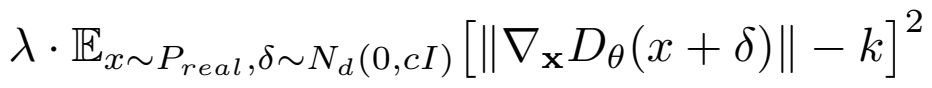
\includegraphics[width=1\linewidth]{img//genAdvNet//modernGAN/dragan_gp.png}
    
As you can see, the formula is very similar, especially since the
authors use \(k = 1\) for their experiments. The main difference with
the WGAN-GP gradient penalty is the \(\delta\) term, which is a noise
term. In their implementation, the authors calculate \(X_p = X + \delta\) as follow:

\[X_{p} = X + 0.5 * \sigma({X}) * N\]

where \(\sigma\) is the standard deviation and \(N\) a noise term
sampled from the uniform distribution. \newline

The gradient penalty is then calculated as follow: 
\begin{itemize}
    \item sample a random point \(\hat{x}\) between the real distribution \(X\) and \(X_{p}\) .
    \item run this sample through the discriminator and calculate the gradient \(\nabla_{\hat{x}} D(\hat{x})\)
    \item calculate the L2 norm of the gradient \(|| \nabla_{\hat{x}} D(\hat{x}) ||_{2}\)
    \item remove 1, square the result and calculate the mean \((|| \nabla_{\hat{x}} D(\hat{x}) ||_{2} - 1) ^{2}\)
\end{itemize}

\subsubsection{BCE Loss}
Interestingly, using this gradient penalty lifts some of the constraint
on the BCE Loss and the author use the above gradient penalty with the
vanilla GAN losses (BCE Loss).

\subsubsection{Third exercise: implement the DRAGAN gradient penalty}

In the third exercise of this notebook, you will implement the DRAGAN
gradient penalty. This is a one liner difference with the above
implementation!

\begin{lstlisting}[language=Python]
def gradient_penalty_dragan(real_sample: torch.Tensor, critic: nn.Module) -> torch.Tensor:
    """
    Gradient penalty of the WGAN-GP model
    args:
    - real_sample: sample from the real dataset
    
    returns:
    - gradient penalty
    """
    # sample a random point between both distributions
    X_p = real_sample + 0.5 * real_sample.std() * torch.rand_like(real_sample)
    
    alpha = torch.rand(real_sample.shape)
    x_hat = alpha * real_sample + (1 - alpha) * X_p
    
    # calculate the gradient
    x_hat.requires_grad = True
    pred = critic(x_hat)
    grad = torch.autograd.grad(pred, 
                               x_hat, 
                               grad_outputs=torch.ones_like(pred), 
                               create_graph=True)[0]
    
    # calculate the norm and the final penalty
    norm = torch.norm(grad.view(-1), 2)
    gp = ((norm - 1)**2).mean()
    return gp
\end{lstlisting}

\begin{lstlisting}[language=Python]
dragan_gp = gradient_penalty_dragan(real_sample, critic)
\end{lstlisting}

\section{WARNING}

The gradient penalty terms penalize each input to the critic
individually. Therefore, the critic should a single input to a single
output. However, we use some layers in the discriminator that remove
this property: the BatchNormalization layers. The authors of the WGAN-GP
paper explain the following:

\begin{quote}
No critic batch normalization Most prior GAN implementations use batch normalization in both the generator and the discriminator to help stabilize training, but batch normalization
changes the form of the discriminator’s problem from mapping a single input to a single output to
mapping from an entire batch of inputs to a batch of outputs . Our penalized training objective
is no longer valid in this setting, since we penalize the norm of the critic’s gradient with respect
to each input independently, and not the entire batch. To resolve this, we simply omit batch normalization in the critic in our models, finding that they perform well without it. Our method works
with normalization schemes which don’t introduce correlations between examples. In particular, we
recommend layer normalization as a drop-in replacement for batch normalization.
\end{quote}

Keep this in mind if you decide to use the gradient penalty in your
project!
